\documentclass[11pt,a4paper]{article}

\usepackage[utf8]{inputenc}
\usepackage[T1]{fontenc}
\usepackage[spanish, es-nodecimaldot]{babel}
\addto\captionsspanish{\renewcommand{\tablename}{Tabla}}
\usepackage{geometry}
\geometry{margin=2.5cm}
\usepackage{booktabs}
\usepackage{array}
\usepackage{multirow}
\usepackage{hyperref}
\hypersetup{colorlinks=true, linkcolor=black, urlcolor=blue}
\usepackage{parskip}
\usepackage{listings}
\usepackage{xcolor}
\usepackage{enumitem}
\usepackage{graphicx}
\usepackage{url}
\graphicspath{{diagrams/}}
\usepackage{float}
\usepackage{caption}
\usepackage{rotating}
\usepackage{pdflscape}
\usepackage{colortbl}
\usepackage{amssymb}
\usepackage{inconsolata}
\usepackage{color}
\usepackage{mdframed}

% ---- Colores --------------------------------------------------
\definecolor{pblue}{rgb}{0.13,0.13,1}
\definecolor{pgreen}{rgb}{0,0.5,0}
\definecolor{pred}{rgb}{0.9,0,0}
\definecolor{pgrey}{rgb}{0.46,0.45,0.48}

\definecolor{lightgray}{gray}{0.92}
\definecolor{codered}{RGB}{180,30,30}
\definecolor{codegreen}{RGB}{0,120,0}
\definecolor{codegray}{RGB}{100,100,100}
\definecolor{warnorange}{RGB}{200,100,0}
\definecolor{noteblue}{RGB}{230,240,255}
\definecolor{noteborder}{RGB}{100,140,200}

% ---- lstset (idéntico al de rediseno-potenciales) -------------
\lstset{
  language=Java,
  basicstyle=\ttfamily\footnotesize,
  keywordstyle=\color{pblue},
  commentstyle=\color{codegray}\itshape,
  stringstyle=\color{pred},
  showstringspaces=false,
  showspaces=false,
  showtabs=false,
  breaklines=true,
  breakatwhitespace=false,
  postbreak=\mbox{\textcolor{codegray}{$\hookrightarrow$}\space},
  frame=single,
  framesep=4pt,
  xleftmargin=6pt,
  xrightmargin=6pt,
  aboveskip=6pt,
  belowskip=6pt,
  numbers=left,
  numberstyle=\tiny\color{codegray},
  numbersep=5pt,
  captionpos=b,
  moredelim=[il][\textcolor{pgrey}]{$$},
  moredelim=[is][\textcolor{pgrey}]{\%\%}{\%\%}
}
\renewcommand{\lstlistingname}{Listado}

% ---- Entorno de nota lateral ----------------------------------
\newmdenv[
  backgroundcolor=noteblue,
  linecolor=noteborder,
  linewidth=1pt,
  innertopmargin=6pt,
  innerbottommargin=6pt,
  innerleftmargin=8pt,
  innerrightmargin=8pt,
  skipabove=8pt,
  skipbelow=8pt,
]{nota}

% ---- Comandos de texto ----------------------------------------
\newcommand{\code}[1]{\texttt{#1}}
\setlength{\emergencystretch}{3em}
\newcommand{\bad}[1]{\textcolor{codered}{\textbf{#1}}}
\newcommand{\good}[1]{\textcolor{codegreen}{\textbf{#1}}}
\newcommand{\warn}[1]{\textcolor{warnorange}{\textbf{#1}}}

% ---------------------------------------------------------------
\title{Evolución de la clase \code{ProbNet}\\[4pt]
       \large Del diagnóstico al rediseño: proceso, decisiones y lecciones\\[4pt]
       \normalsize \code{org.openmarkov.core} --- paquete \code{model.network}}
\author{Manuel Arias}
\date{Abril de 2026}
% ---------------------------------------------------------------

\begin{document}

\maketitle
\tableofcontents
\newpage

% ===================================================================
\section{Fundamentos de ingeniería del software}
\label{sec:fundamentos}

Esta sección define los conceptos de ingeniería del software que se
aplican a lo largo del documento.  Es especialmente útil para lectores
con poca experiencia en diseño orientado a objetos: los términos técnicos
se usan con precisión en el resto del texto.

% -------------------------------------------------------------------
\subsection{Principios de diseño}
\label{sec:principios}

Los \emph{principios de diseño} son reglas generales que, cuando se
aplican con criterio, producen código más fácil de entender, modificar y
probar.  No son leyes inmutables: su valor está en que obligan a
\emph{justificar} por escrito las decisiones de diseño.

\paragraph{Principio de Responsabilidad Única (SRP).}
\label{sec:srp}
Una clase debe tener \textbf{una sola razón para cambiar}~\cite{martin2003}.
Si un módulo hace demasiadas cosas a la vez, cualquier modificación en una
de ellas obliga a revisar y re-probar todas las demás.  El indicador más
claro de que una clase viola el SRP es que necesita importaciones de
paquetes que ``no le corresponden'': si el modelo de dominio importa
clases de I/O, algo va mal.

\paragraph{Principio DRY (\emph{Don't Repeat Yourself}).}
\label{sec:dry}
Cada pieza de conocimiento debe tener \textbf{una única representación}
en el sistema~\cite{hunt1999}.  Cuando la misma lógica aparece en dos
lugares, una corrección debe aplicarse en ambos; si se olvida uno, el
comportamiento queda inconsistente.

\paragraph{Principio de Inversión de Dependencias (DIP).}
\label{sec:dip}
Los módulos de alto nivel (el modelo de dominio) \textbf{no deben depender
de los módulos de bajo nivel} (I/O, persistencia)~\cite{martin2003}.
Ambos deben depender de abstracciones.  Si el modelo sabe cómo leer y
escribir ficheros, un cambio de formato puede obligar a tocar la parte
más delicada del sistema.

\paragraph{Composición frente a herencia.}
\label{sec:composicion}
Existen dos formas de reutilizar comportamiento en programación orientada
a objetos: la \emph{herencia} (``B es un tipo de A'') y la
\emph{composición} (``B \emph{tiene} un objeto de tipo A'').  La herencia
crea un acoplamiento muy fuerte: la subclase hereda \emph{todo} lo del
padre, incluyendo lo que no necesita, y cualquier cambio en el padre puede
romper la subclase.  Un principio clásico recomienda \textbf{preferir la
composición} siempre que la relación no sea genuinamente ``es un tipo
de''~\cite{gamma1995}.

\paragraph{Principio de Segregación de Interfaces (ISP).}
\label{sec:isp}
Una clase no debe ser obligada a depender de métodos que no utiliza.  Es
preferible tener \textbf{varias interfaces pequeñas y específicas} que una
sola interfaz grande~\cite{martin2003}: así, cada consumidor declara
exactamente las capacidades que necesita.  Un algoritmo de inferencia que
solo consulta el grafo no debería necesitar importar una clase con 80
métodos.

% -------------------------------------------------------------------
\subsection{Antipatrones detectados}
\label{sec:antipatrones}

Un \emph{antipatrón} es un patrón de diseño que, en apariencia razonable,
genera en la práctica problemas de mantenimiento.  Reconocerlos en el
propio código es la mitad del trabajo.

\paragraph{God Class (Clase Dios).}
Una clase que acumula demasiadas responsabilidades: lo sabe todo y lo hace
todo~\cite{fowler2019}.  Sus síntomas son: cientos o miles de líneas,
métodos de dominios no relacionados y muchas dependencias entrantes (todo
el sistema pasa por ella).  Es dañina porque viola el SRP, hace imposibles
las pruebas unitarias aisladas y se convierte en el cuello de botella del
desarrollo.

\paragraph{Herencia inapropiada.}
Usar herencia para reutilizar la implementación de otra clase aunque la
relación ``es un tipo de'' no sea semánticamente correcta.  El resultado
es que la subclase hereda métodos y campos que no le corresponden y queda
atada a todos los cambios del padre.  La solución es sustituir la herencia
por composición y declarar las capacidades mediante interfaces.

% -------------------------------------------------------------------
\subsection{Patrones de diseño aplicados}
\label{sec:patrones}

\paragraph{Extract Class (Extraer Clase).}
Cuando una clase tiene demasiadas responsabilidades, se identifica un grupo
cohesivo de métodos y campos y se mueve a una nueva clase~\cite{fowler2019}.
La clase original delega en la nueva.  Este patrón no cambia el
comportamiento externo: si se aplica correctamente, los tests existentes
siguen pasando sin modificación alguna.

\paragraph{Value Object (Objeto Valor).}
Un objeto que agrupa datos relacionados sin identidad propia: lo que
importa es su contenido, no su dirección en memoria.  Útil para separar
los datos de configuración del comportamiento de dominio.

\paragraph{Interfaces como contrato mínimo.}
En lugar de hacer que todo el código cliente dependa de una clase concreta
grande, se definen interfaces que describen solo las capacidades que cada
cliente necesita.  La clase concreta implementa todas las interfaces
aplicables.  El cliente declara su dependencia sobre la interfaz: si
mañana cambia la implementación, el cliente no necesita modificarse.

% ===================================================================
\section{El punto de partida: por qué \texttt{ProbNet} necesitaba cambiar}
\label{sec:punto-partida}

\subsection{Una clase de importancia crítica}

\code{ProbNet} es la clase más referenciada de OpenMarkov.
\textbf{490~ficheros} la importan en alguna de sus formas.  Representa la
red probabilística en sí misma: sus nodos, arcos, potenciales,
restricciones y metadatos.  Sin ella, el proyecto no existe.

Precisamente por su centralidad, \code{ProbNet} fue acumulando
responsabilidades durante años.  En el momento del análisis, la clase
tenía \textbf{1440~líneas}, \textbf{más de 80~métodos públicos} y
cubría seis áreas de responsabilidad completamente distintas:

\begin{enumerate}[nosep]
  \item Gestión de nodos, arcos y variables.
  \item Gestión de potenciales (tablas de probabilidad y utilidad).
  \item Restricciones de la red.
  \item Clasificación de la red (¿es temporal? ¿multiagente? ¿solo nodos chance?).
  \item Gestión de agentes.
  \item Metadatos descriptivos e I/O (nombre, comentario, lector/escritor de ficheros).
\end{enumerate}

Cada una de estas áreas tiene su propia razón para cambiar.  Un bug en la
gestión de agentes no tiene nada que ver con la lógica de potenciales, pero
en el mismo fichero ambas convivían.  Esto es la definición de God Class
(§\ref{sec:antipatrones}).

\subsection{La herencia directa de \texttt{Graph}}

\code{ProbNet} extendía \code{Graph<Node>}, la clase genérica de grafo
de la librería interna.  Esta elección de diseño tuvo sentido en su
momento, pero con el tiempo generó dos problemas:

\begin{itemize}
  \item \code{ProbNet} exponía la API completa de \code{Graph}: métodos
        como \code{addVertex()} y \code{removeVertex()} (operaciones de
        bajo nivel del grafo genérico) formaban parte del contrato público
        de la red probabilística.  No había forma de distinguir las
        operaciones de dominio de las de infraestructura.

  \item No existía ninguna interfaz que permitiera a un algoritmo declarar
        que solo necesitaba \emph{consultar} la red.  Todo el código que
        quería consultar la topología debía aceptar \code{ProbNet} completa,
        con sus 80~métodos, aunque solo usase tres.  Esto viola el ISP y el
        DIP (§\ref{sec:principios}).
\end{itemize}

\subsection{La acumulación de deuda técnica}

La situación no era el resultado de malas decisiones puntuales, sino de
una acumulación gradual de deuda técnica.  Cada nueva funcionalidad se
añadía donde más cómodo resultaba --- en \code{ProbNet}, porque ya tenía
acceso a todo.  Esta es la dinámica habitual de las God Classes: no nacen
grandes; crecen.

Al momento del análisis, la deuda era cuantificable:

\begin{center}
\begin{tabular}{lr}
\toprule
\textbf{Métrica} & \textbf{Valor} \\
\midrule
Líneas de código                & 1\,440 \\
Métodos públicos                & 80+ \\
Campos                          & 16 \\
Ficheros dependientes           & 490 \\
Áreas de responsabilidad        & 6 \\
Bugs conocidos                  & 4 \\
Code smells documentados        & 7 \\
Cobertura de tests (métodos)    & 37\% \\
\bottomrule
\end{tabular}
\end{center}

% ===================================================================
\section{El diagnóstico}
\label{sec:diagnostico}

El primer paso fue documentar con precisión la situación existente, sin
empezar a cambiar nada todavía.  La Figura~\ref{fig:actual} muestra el
diagrama resultante.

\begin{figure}[H]
  \centering
  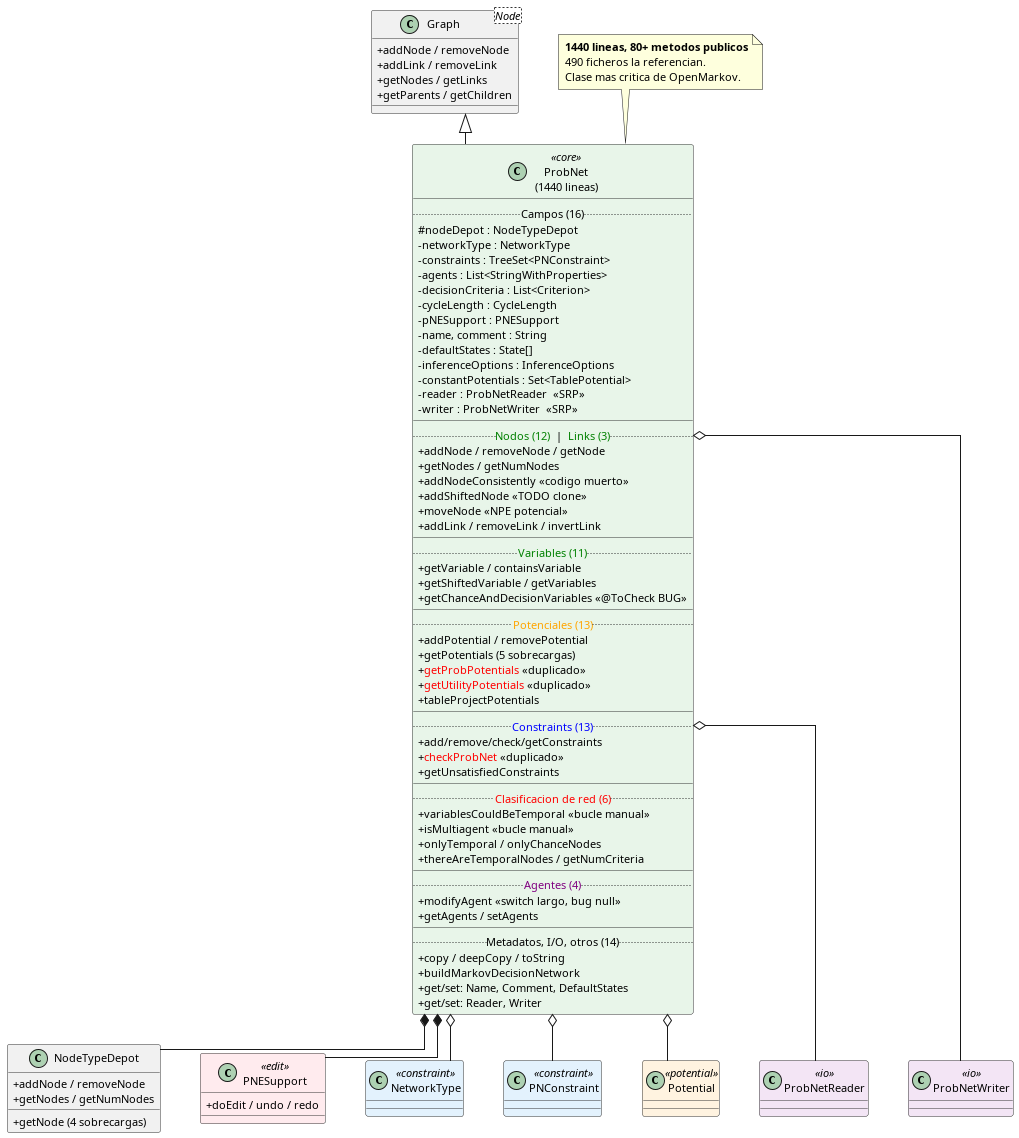
\includegraphics[width=\textwidth]{probnet-actual.png}
  \caption{Diagrama UML de \code{ProbNet} antes del rediseño.  Los colores
           agrupan las seis áreas de responsabilidad; las etiquetas en rojo
           señalan los problemas.}
  \label{fig:actual}
\end{figure}

\code{ProbNet} extendía \code{Graph<Node>} y añadía:
\begin{itemize}[nosep]
  \item \textbf{16~campos}: desde \code{nodeDepot} (indexación de nodos
        por tipo) hasta \code{reader}/\code{writer} (I/O).
  \item \textbf{80+~métodos públicos}: gestión de nodos (12), links (3),
        variables (11), potenciales (13), constraints (13), clasificación
        de red (6), agentes (4), metadatos e I/O (12), y otros (copia,
        inferencia, criterios).
\end{itemize}

% -------------------------------------------------------------------
\subsection{Los bugs confirmados}
\label{sec:bugs}

La Figura~\ref{fig:bugs} resume los bugs, code smells y riesgos
identificados.

\begin{figure}[H]
  \centering
  
\includegraphics[width=\textwidth]{bugs-detectados.png}
  \caption{Bugs confirmados (\textcolor{codered}{rojo}), code smells
           (\textcolor{warnorange}{amarillo}) y riesgos de tipo
           (\textcolor{warnorange}{naranja}) en \code{ProbNet}.}
  \label{fig:bugs}
\end{figure}

\subsubsection{B1: \texttt{getChanceAndDecisionVariables()} incluye tipos extra}

El método está anotado con \code{@ToCheck(PROBABLE\_BUG)}.  Su nombre
indica que devuelve solo variables de tipo CHANCE y DECISION, pero el
\code{switch} también incluye \code{SV\_PRODUCT} y \code{SV\_SUM}:

\begin{lstlisting}[caption={B1: el \texttt{switch} incluye tipos no mencionados en el nombre.},
                   label=lst:b1]
case CHANCE, SV_PRODUCT, SV_SUM, DECISION -> true;
case UTILITY -> false;
\end{lstlisting}

Si el comportamiento actual es intencionado, el nombre del método es
engañoso.  Si no lo es, devuelve variables de más.

\subsubsection{B2: \texttt{moveNode()} --- NullPointerException potencial}

En la línea~1389, \code{getNode(name)} puede devolver \code{null} si el
nombre no existe en la red.  No hay comprobación de nulidad antes de usar
el resultado:

\begin{lstlisting}[caption={B2: acceso sin null-check sobre el resultado de \texttt{getNode()}.},
                   label=lst:b2]
Node node = getNode(name);
// NPE aqui si name no existe en la red:
node.setCoordinateX(newPositions.get(i).getX());
node.setCoordinateY(newPositions.get(i).getY());
\end{lstlisting}

\subsubsection{B3: \texttt{modifyAgent(REMOVE)} deja \texttt{agents = null}}

Cuando se elimina el último agente, el método asigna
\code{agents = null}:

\begin{lstlisting}[caption={B3: la asignación \texttt{agents = null} causa NPE posterior.},
                   label=lst:b3]
case REMOVE -> {
    for (int i = 0; i < agents.size(); i++) {
        if (agents.get(i).getString().equals(agentName)) {
            agents.remove(i);
        }
    }
    if (agents.size() == 0) {
        agents = null;  // <-- cualquier llamada posterior a
    }                   //     getAgents() causa NPE
    // ...
}
\end{lstlisting}

\code{getAgents()} devuelve el campo directamente sin comprobar nulidad,
por lo que cualquier iteración posterior lanza \code{NullPointerException}.
Además, \code{modifyAgent(ADD)} crea la lista si es \code{null}, pero
nunca debería haberlo sido.

\subsubsection{B4: \texttt{addShiftedNode()} no copia potenciales}

El método copia el tipo de nodo, coordenadas, propósito, relevancia,
comentario y propiedades adicionales, pero \textbf{no copia los
potenciales} del nodo original ni crea uno por defecto.  El propio
código reconoce el problema con un comentario \code{TODO}:

\begin{lstlisting}[caption={B4: potenciales no copiados; el TODO reconoce la deuda.},
                   label=lst:b4]
// TODO Hacer clon para node y quitar estas lineas
node.setNodeType(originalNode.getNodeType());
node.setCoordinateX(originalNode.getCoordinateX() + shiftX);
node.setCoordinateY(originalNode.getCoordinateY() + shiftY);
node.setPurpose(originalNode.getPurpose());
// ... propiedades copiadas ...
// Potenciales: NO se copian (omision confirmada)
\end{lstlisting}

% -------------------------------------------------------------------
\subsection{Los code smells}
\label{sec:smells}

\subsubsection{S1: Lógica duplicada entre \texttt{checkProbNet()} y
                   \texttt{getUnsatisfiedConstraints()} (violación DRY)}

Ambos métodos iteraban sobre \code{constraints} con la misma condición
\code{constraint.isMetBy(this)}.  Si la lógica de verificación cambiaba,
había que actualizar dos métodos:

\begin{lstlisting}[caption={S1: el mismo bucle aparece en dos métodos (violación DRY).},
                   label=lst:s1-antes]
public boolean checkProbNet() {
    for (PNConstraint constraint : constraints) {
        if (!constraint.isMetBy(this)) { return false; }
    }
    return true;
}

public List<PNConstraint> getUnsatisfiedConstraints() {
    List<PNConstraint> unsatisfied = new ArrayList<>();
    for (PNConstraint constraint : constraints) {
        if (!constraint.isMetBy(this)) {
            unsatisfied.add(constraint);
        }
    }
    return unsatisfied;
}
\end{lstlisting}

\subsubsection{S2: Bucles manuales en clasificación de red}

\code{variablesCouldBeTemporal()} e \code{isMultiagent()} usaban un
bucle \code{for} manual sobre \code{constraints} con \code{instanceof},
cuando ya existía \code{hasConstraintOfClass()} que hace exactamente eso:

\begin{lstlisting}[caption={S2: bucle manual donde existe un método más expresivo.},
                   label=lst:s2]
// Antes (7 lineas con logica que hasConstraintOfClass() ya encapsula):
public boolean variablesCouldBeTemporal() {
    for (PNConstraint constraint : constraints) {
        if (constraint instanceof OnlyAtemporalVariables) return false;
    }
    return true;
}

// Despues (1 linea, aprovechando el metodo existente):
public boolean variablesCouldBeTemporal() {
    return !hasConstraintOfClass(OnlyAtemporalVariables.class);
}
\end{lstlisting}

\subsubsection{S3: Patrón duplicado entre \texttt{getProbPotentials()} y
                   \texttt{getUtilityPotentials()} (violación DRY)}

Ambos métodos seguían el mismo algoritmo: obtener el nodo de la variable,
reunir vecinos, iterar potenciales y filtrar por rol.  Solo difería el
predicado de filtro (\code{CONDITIONAL\_PROBABILITY} frente a
\code{UTILITY}).  Con 40~líneas de código duplicadas, un error en el
algoritmo de búsqueda debería corregirse en dos sitios.

\subsubsection{S4: \texttt{getNumCriteria()} con complejidad
                   \texorpdfstring{$O(n \cdot m)$}{O(n*m)}}

El método usaba una \code{List<String>} con búsqueda lineal para detectar
duplicados:

\begin{lstlisting}[caption={S4: complejidad cuadrática innecesaria con \texttt{List}.},
                   label=lst:s4]
// Antes: List + contains() = O(n*m)
List<String> criteriaNames = new ArrayList<>();
for (Potential potential : getPotentials(PotentialRole.UTILITY)) {
    String name = potential.getCriterion().toString();
    if (!criteriaNames.contains(name)) { // busqueda lineal
        criteriaNames.add(name);
    }
}
return criteriaNames.size();

// Despues: Set = O(n log n)
Set<String> criteriaNames = new TreeSet<>();
getPotentials(PotentialRole.UTILITY).forEach(
    p -> criteriaNames.add(p.getCriterion().toString()));
return criteriaNames.size();
\end{lstlisting}

\subsubsection{S5: Código comentado e \texttt{if}-chain en
                   \texttt{addNodeConsistently()}}

Las líneas 933--938 contenían 6~líneas de código comentado que nunca se
ejecutaban.  Además, el método usaba una cadena de \code{if} en lugar de
\code{switch}, lo que dificulta la lectura cuando hay más de tres ramas.

\subsubsection{S6: \texttt{toString()} en la línea~53}

El método \code{toString()} estaba ubicado al inicio del fichero, antes
incluso de la declaración de los campos.  La convención en Java es:
campos $\to$ constructores $\to$ métodos de instancia $\to$ métodos
auxiliares.  Colocar \code{toString()} al principio sugiere que fue
añadido puntualmente para depuración y nunca se reubicó.

\subsubsection{S7: \texttt{reader}/\texttt{writer} en el modelo de dominio
                   (violación SRP y DIP)}

\code{ProbNet} almacenaba referencias a \code{ProbNetReader} y
\code{ProbNetWriter}, los objetos responsables de la lectura y escritura
de ficheros en disco.  El motivo era funcional: la GUI necesitaba saber
con qué formato se había abierto la red para usar el mismo formato al
guardar.  Sin embargo, esa información pertenece al controlador de
ficheros, no al modelo de dominio.  Esta violación del DIP acoplaba el
módulo \code{core} con los módulos \code{io} y \code{gui}.

% -------------------------------------------------------------------
\subsection{Cobertura de tests}
\label{sec:cobertura}

Las Figuras~\ref{fig:cob-nlv}, \ref{fig:cob-pc} y~\ref{fig:cob-cai}
muestran el estado de la cobertura de tests por área funcional.

\begin{figure}[H]
  \centering
  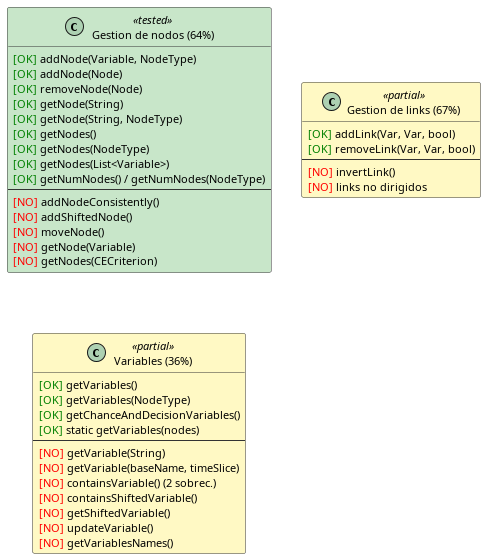
\includegraphics[width=0.7\textwidth]{cobertura-nodos-links-vars.png}
  \caption{Cobertura de tests: nodos (64\%), links (67\%) y variables
           (36\%).}
  \label{fig:cob-nlv}
\end{figure}

\begin{figure}[H]
  \centering
  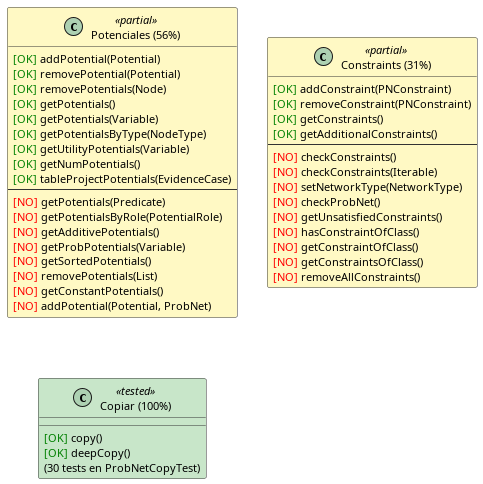
\includegraphics[width=0.7\textwidth]{cobertura-potenciales-constraints.png}
  \caption{Cobertura de tests: potenciales (56\%), constraints (31\%)
           y copia (100\%).}
  \label{fig:cob-pc}
\end{figure}

\begin{figure}[H]
  \centering
  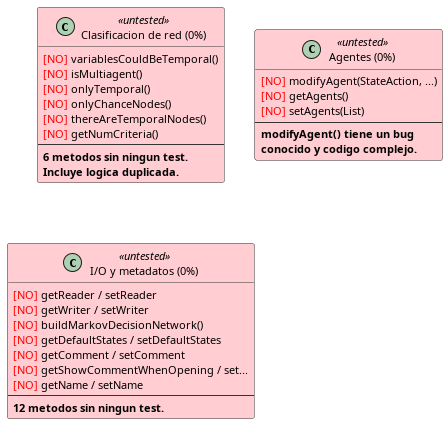
\includegraphics[width=0.7\textwidth]{cobertura-clasificacion-agentes-io.png}
  \caption{Cobertura de tests: clasificación de red (0\%), agentes (0\%)
           e I/O y metadatos (0\%).  Estas tres áreas eran las lagunas
           más críticas.}
  \label{fig:cob-cai}
\end{figure}

\subsubsection{Resumen cuantitativo}

\begin{center}
\begin{tabular}{lccr}
\toprule
\textbf{Área} & \textbf{Métodos} & \textbf{Testados} & \textbf{Cobertura} \\
\midrule
Gestión de nodos        & 14 & 9  & 64\% \\
Gestión de links        & 3  & 2  & 67\% \\
Variables               & 11 & 4  & 36\% \\
Potenciales             & 16 & 9  & 56\% \\
Constraints             & 13 & 4  & 31\% \\
Clasificación de red    & 6  & 0  & \bad{0\%} \\
Agentes                 & 4  & 0  & \bad{0\%} \\
Copiar                  & 2  & 2  & 100\% \\
I/O y metadatos         & 12 & 0  & \bad{0\%} \\
\midrule
\textbf{Total}          & \textbf{81} & \textbf{30} & \textbf{37\%} \\
\bottomrule
\end{tabular}
\end{center}

Existían \textbf{30~tests} en \code{ProbNetTest} y \textbf{30~tests} en
\code{ProbNetCopyTest}, pero \textbf{51~métodos públicos} no tenían
ningún test unitario directo.

La ausencia total de tests en clasificación, agentes y metadatos no es
una coincidencia: son exactamente las áreas donde vivían los bugs B1, B3
y el smell S7.  Hay una relación circular entre God Class y ausencia de
tests: una clase grande con muchas responsabilidades es difícil de aislar
para probar, y sin tests la cobertura baja, lo que hace más difícil
detectar bugs y más arriesgado refactorizar.

% ===================================================================
\section{La hoja de ruta: diseñar el cambio antes de ejecutarlo}
\label{sec:hoja-ruta}

\subsection{El principio rector: retrocompatibilidad total}

Con 490~ficheros dependientes, la tentación es hacer un rediseño ``de una
sola vez'' que resuelva todo al mismo tiempo.  Esa estrategia es
arriesgada: cualquier error rompe todo y puede ser difícil de localizar.

Se adoptó el principio de que \textbf{cada fase debe dejar el sistema
funcionando}: al final de cada fase, todos los tests deben pasar.  Esto
convierte el proceso en una sucesión de pasos seguros, cada uno
verificable de forma independiente.

La técnica que hace posible este principio es la
\textbf{delegación retrocompatible}: cuando se extrae un método a una
clase nueva, no se elimina de \code{ProbNet}.  En su lugar, el método
original se convierte en una llamada a la nueva clase:

\begin{lstlisting}[caption={Patrón de delegación retrocompatible.},
                   label=lst:retro]
// ProbNet.java ANTES:
public boolean isMultiagent() {
    for (PNConstraint constraint : constraints) {
        if (constraint instanceof OnlyOneAgent) return false;
    }
    return true;
}

// ProbNet.java DESPUES de extraer ProbNetClassifier:
public boolean isMultiagent() {
    return ProbNetClassifier.isMultiagent(this); // delega
}
\end{lstlisting}

El código que llama a \code{probNet.isMultiagent()} \textbf{no necesita
cambiar nada}.  La refactorización es invisible para los consumidores de
la clase.

\subsection{La arquitectura objetivo}

La Figura~\ref{fig:propuesta} muestra el objetivo planteado al final del
análisis.

\begin{figure}[H]
  \centering
  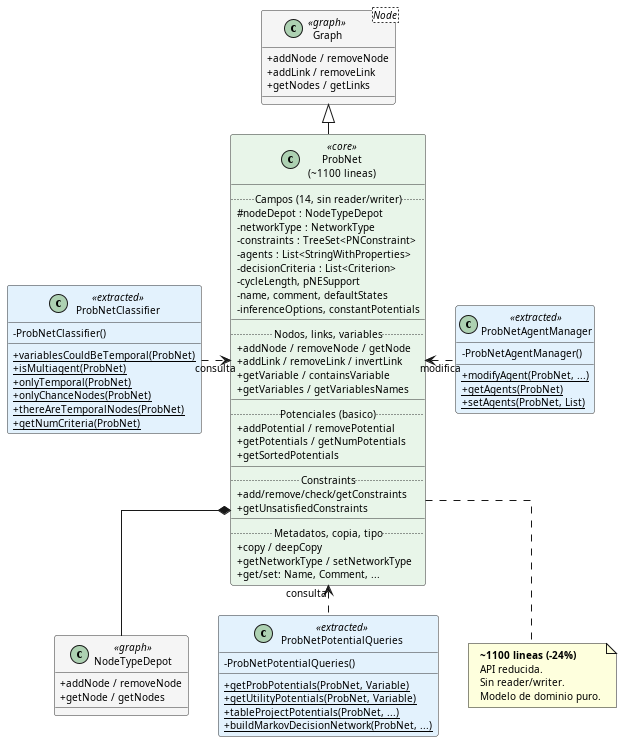
\includegraphics[width=\textwidth]{probnet-propuesta.png}
  \caption{Arquitectura propuesta al inicio del proceso.  Se identificaron
           tres extracciones principales; la ejecución añadió dos más.}
  \label{fig:propuesta}
\end{figure}

La propuesta inicial identificaba tres grupos claros para extracción:
clasificación de la red, gestión de agentes y consultas de potenciales.
Durante la ejecución se añadieron dos más (\code{NetworkMetadata} y
\code{ProbNetCopier}) y se ejecutó el cambio más profundo: la sustitución
de la herencia por composición con interfaces.

\subsection{Fase 0: ampliar los tests (prerrequisito)}
\label{sec:fase0}

Antes de cualquier refactorización, era necesario cubrir las lagunas
críticas de cobertura.  Sin tests, la refactorización es potencialmente
destructiva; con tests, es un proceso predecible.

\begin{center}
\footnotesize
\begin{tabular}{lp{8.5cm}r}
\toprule
\textbf{Área} & \textbf{Tests a añadir} & \textbf{Prioridad} \\
\midrule
Variables   & \code{getVariable}, \code{containsVariable},
              \code{getShiftedVariable}, \code{getVariablesNames},
              \code{updateVariable} & Alta \\
Constraints & \code{setNetworkType} (cambio válido e inválido con
              rollback), \code{checkProbNet},
              \code{getUnsatisfiedConstraints},
              \code{hasConstraintOfClass} & Alta \\
Clasificación & Todos los 6~métodos con redes BN, ID y DBN & Alta \\
Agentes     & \code{modifyAgent} ADD/REMOVE/RENAME con casos límite & Alta \\
Potenciales & \code{addPotential(pot, origNet)},
              \code{getProbPotentials}, \code{getSortedPotentials},
              \code{getConstantPotentials} & Media \\
Nodos       & \code{moveNode} (normal y nombre inválido),
              \code{addShiftedNode}, \code{invertLink} & Media \\
Metadatos   & \code{getDefaultStates}, \code{comment},
              \code{showCommentWhenOpening} & Baja \\
\bottomrule
\end{tabular}
\end{center}

Objetivo: pasar de \textbf{37\%} a \textbf{$>$80\%} de cobertura de
métodos públicos antes de empezar las extracciones.

\subsection{Las fases y su riesgo estimado}

\begin{center}
\begin{tabular}{clcc}
\toprule
\textbf{Fase} & \textbf{Descripción} & \textbf{Riesgo} & \textbf{Dependencia} \\
\midrule
0 & Ampliar tests                    & Bajo  & --- \\
1 & Corregir bugs y code smells      & Bajo  & Fase~0 \\
  & Extraer \code{NetworkMetadata}   & Bajo  & Fase~0 \\
  & Extraer \code{ProbNetCopier}     & Bajo  & Fase~0 \\
3 & Extraer \code{ProbNetClassifier} & Medio & Fase~0, 1 \\
4 & Extraer \code{ProbNetAgentManager} & Bajo & Fase~0, 1 \\
5 & Extraer \code{ProbNetPotentialQueries} & Medio & Fase~0 \\
  & Herencia $\to$ composición + interfaces & Alto & Fase~0 \\
6 & Evaluar mover \code{reader}/\code{writer} a la GUI & Alto & Fase~0 \\
\bottomrule
\end{tabular}
\end{center}

Las fases 0--1 son de bajo riesgo y alto valor.  Las fases 3--5 siguen el
patrón \emph{Extract Class} ya probado con éxito en
\code{VariableStateOperations} y \code{VariableTypeConverter}.  La fase~6
requiere un análisis de impacto en los módulos \code{gui} e \code{io}.

% ===================================================================
\section{La ejecución del rediseño}
\label{sec:ejecucion}

\subsection{El estado real de partida}

La Figura~\ref{fig:before} muestra la estructura interna de
\code{ProbNet} agrupada por área de responsabilidad, con el color de cada
sección indicando el dominio.

\begin{figure}[H]
  \centering
  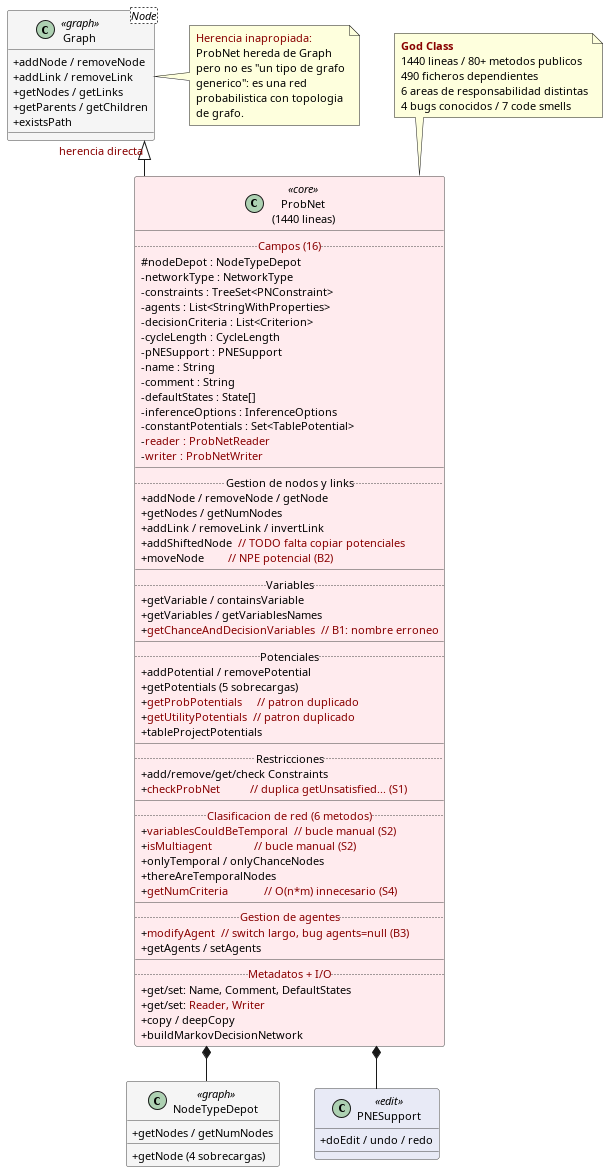
\includegraphics[width=0.85\textwidth]{before.png}
  \caption{Estructura interna de \code{ProbNet} al inicio del rediseño.}
  \label{fig:before}
\end{figure}

\subsection{Fase 1: corregir bugs y simplificaciones}
\label{sec:fase1-exec}

Los cuatro bugs y los siete code smells se resolvieron sin modificar la
API pública.

\paragraph{Bug B1 --- Renombrar \texttt{getChanceAndDecisionVariables()}.}
El análisis del uso en el proyecto confirmó que los tipos
\code{SV\_PRODUCT}/\code{SV\_SUM} debían incluirse, porque los llamadores
esperaban ese comportamiento.  El problema era el nombre: se renombró a
\code{getNonUtilityVariables()}, que describe con precisión lo que el
método hace.  Se conservó el nombre antiguo como método \code{@Deprecated}
para compatibilidad.

\paragraph{Bug B2 --- Null-check en \texttt{moveNode()}.}
Se añadió una comprobación explícita: si \code{getNode(name)} devuelve
\code{null}, el método ignora ese nombre en lugar de lanzar una excepción.

\paragraph{Bug B3 --- Inicializar \texttt{agents} con lista vacía.}
Se eliminó la asignación \code{agents = null} en
\code{modifyAgent(REMOVE)}.  La lista se inicializa como vacía desde el
principio y nunca se asigna \code{null}.  Esto garantiza que
\code{getAgents()} siempre devuelve una lista (posiblemente vacía), nunca
\code{null}.

\paragraph{Bug B4 --- \texttt{addShiftedNode()} sin potenciales.}
La resolución queda pendiente porque requiere decidir qué comportamiento
esperan los llamadores: ¿copiar los potenciales del nodo original, o crear
un potencial uniforme por defecto?  Se añadió un test que documenta el
comportamiento actual y el comentario \code{@ToCheck}.

\paragraph{Code smells S1--S7.}
\begin{itemize}[nosep]
  \item S1: \code{checkProbNet()} reducido a
        \code{getUnsatisfiedConstraints().isEmpty()} (DRY).
  \item S2: \code{variablesCouldBeTemporal()} e \code{isMultiagent()}
        usan ahora \code{hasConstraintOfClass()}.
  \item S3: patrón duplicado resuelto al extraer
        \code{ProbNetPotentialQueries} (§\ref{sec:potqueries}).
  \item S4: \code{getNumCriteria()} usa ahora un \code{TreeSet}.
  \item S5: eliminado el código comentado y convertida la cadena
        \code{if} en \code{switch} en \code{addNodeConsistently()}.
  \item S6: \code{toString()} movido al final del fichero.
  \item S7: \code{reader}/\code{writer} incluidos en
        \code{NetworkMetadata} (§\ref{sec:metadata}) como solución
        intermedia.
\end{itemize}

El listado~\ref{lst:dry} ilustra la corrección del smell S1.

\begin{lstlisting}[caption={S1: \texttt{checkProbNet()} delega en
                            \texttt{getUnsatisfiedConstraints()} (DRY).},
                   label=lst:dry]
// ANTES: 8 lineas duplicando la logica:
public boolean checkProbNet() {
    for (PNConstraint constraint : constraints) {
        if (!constraint.isMetBy(this)) { return false; }
    }
    return true;
}

// DESPUES: 1 linea que reutiliza el metodo existente:
public boolean checkProbNet() {
    return getUnsatisfiedConstraints().isEmpty();
}
\end{lstlisting}

% -------------------------------------------------------------------
\subsection{Extracción de \texttt{NetworkMetadata}}
\label{sec:metadata}

\textbf{Motivación (SRP, §\ref{sec:srp}; Extract Class,
§\ref{sec:patrones}; Value Object, §\ref{sec:patrones}):}
\code{ProbNet} almacenaba directamente once campos de metadatos: nombre,
comentario, si mostrar el comentario al abrir, estados por defecto,
criterios de decisión, agentes, longitud de ciclo, opciones de inferencia,
propiedades adicionales de formato, \code{reader} y \code{writer}.
Estos datos no tienen comportamiento de dominio propio y cambiarán cuando
cambie la interfaz de usuario o el formato de fichero, no cuando cambie
la lógica de inferencia.

\textbf{Decisión:} se extrajeron los 11~campos a un objeto valor
\code{NetworkMetadata} que \code{ProbNet} posee como campo privado.
\code{ProbNet} conserva todos sus \emph{getters} y \emph{setters}
públicos, delegando ahora en \code{NetworkMetadata}.

\begin{lstlisting}[caption={Antes: campos de metadatos directamente en \texttt{ProbNet}.},
                   label=lst:meta-antes]
public class ProbNet extends Graph<Node> {
    private String name;
    private String comment = "";
    private boolean showCommentWhenOpening = false;
    private State[] defaultStates = { ... };
    private InferenceOptions inferenceOptions = new InferenceOptions();
    private CycleLength cycleLength = new CycleLength();
    // ... 5 campos mas de metadatos ...

    public String getName() { return name; }
    public void setName(String name) { this.name = name; }
    // ...
}
\end{lstlisting}

\begin{lstlisting}[caption={Después: metadatos delegados a \texttt{NetworkMetadata}.},
                   label=lst:meta-despues]
public class ProbNet implements PotentialNetwork {
    private final NetworkMetadata metadata = new NetworkMetadata();
    // campos de dominio: grafo, restricciones, potenciales...

    public String getName()              { return metadata.getName(); }
    public void setName(String name)     { metadata.setName(name); }
    public String getComment()           { return metadata.getComment(); }
    public void setComment(String c)     { metadata.setComment(c); }
    // ... todos los demas getters/setters delegan igual ...
}
\end{lstlisting}

El efecto en los campos de \code{ProbNet} fue inmediato: de \textbf{16
campos} pasó a \textbf{7}.  Los 11~campos de metadatos fueron
reemplazados por un único campo \code{metadata}.

La clase \code{NetworkMetadata} resultante agrupa:

\begin{center}
\begin{tabular}{ll}
\toprule
\textbf{Campo} & \textbf{Tipo} \\
\midrule
\code{name}                      & \code{String} \\
\code{comment}                   & \code{String} \\
\code{showCommentWhenOpening}    & \code{boolean} \\
\code{defaultStates}             & \code{State[]} \\
\code{agents}                    & \code{List<StringWithProperties>} \\
\code{decisionCriteria}          & \code{List<StringWithProperties>} \\
\code{cycleLength}               & \code{CycleLength} \\
\code{inferenceOptions}          & \code{InferenceOptions} \\
\code{additionalProperties}      & \code{Map<String, String>} \\
\code{reader}                    & \code{ProbNetReader} \\
\code{writer}                    & \code{ProbNetWriter} \\
\bottomrule
\end{tabular}
\end{center}

\begin{nota}
\textbf{¿Por qué los campos \code{reader}/\code{writer} no se movieron
fuera de \code{ProbNet}?}  La solución correcta al smell S7 sería mover
estos campos al controlador de ficheros de la GUI.  Sin embargo, hacerlo
requiere un análisis de impacto en los módulos \code{gui} e \code{io}
que va más allá del alcance de esta refactorización.  Como solución
intermedia, los campos se incluyen en \code{NetworkMetadata}, donde al
menos quedan claramente identificados como ``datos de sesión'', no como
comportamiento de dominio.  La migración completa está documentada como
tarea pendiente.
\end{nota}

% -------------------------------------------------------------------
\subsection{Extracción de \texttt{ProbNetCopier}}
\label{sec:copier}

\textbf{Motivación (SRP, §\ref{sec:srp}; Extract Class, §\ref{sec:patrones}):}
\code{ProbNet} contenía dos métodos de copia, \code{copy()} y
\code{deepCopy()}, con implementaciones de 40 y 50~líneas
respectivamente.  La lógica es compleja: iterar nodos, arcos, potenciales
y restricciones, y decidir qué se comparte por referencia (copia
superficial) y qué se instancia de nuevo (copia profunda).  Esta lógica
no pertenece al modelo de dominio: el modelo de la red no tiene por qué
saber cómo preparar una copia de sí mismo para inferencia.

\textbf{Decisión:} se extrajo la lógica de copia a \code{ProbNetCopier}
(visibilidad de paquete, no pública).  Los métodos \code{copy()} y
\code{deepCopy()} de \code{ProbNet} permanecen en la API pública como
delegaciones:

\begin{lstlisting}[caption={Extracción de la lógica de copia a \texttt{ProbNetCopier}.},
                   label=lst:copier]
// ProbNet.java (API publica inalterada):
public ProbNet copy() {
    return ProbNetCopier.shallowCopy(this);
}

public ProbNet deepCopy() {
    return ProbNetCopier.deepCopy(this);
}

// ProbNetCopier.java (logica compleja, fuera del dominio):
final class ProbNetCopier {
    private ProbNetCopier() {} // no instanciable

    static ProbNet shallowCopy(ProbNet original) {
        // Copia la estructura compartiendo referencias a
        // Variables y Potentials (semantica "copy"):
        // - nodos nuevos con las mismas Variables (compartidas)
        // - arcos nuevos
        // - potenciales compartidos (no clonados)
        // - restricciones compartidas
        // ... 40 lineas de logica ...
    }

    static ProbNet deepCopy(ProbNet original) {
        // Crea nuevas instancias de todos los objetos mutables:
        // - nodos nuevos con nuevas Variables
        // - nuevos potenciales clonados
        // - nuevas restricciones
        // ... 50 lineas de logica ...
    }
}
\end{lstlisting}

% -------------------------------------------------------------------
\subsection{Extracción de \texttt{ProbNetClassifier}}
\label{sec:classifier}

\textbf{Motivación (SRP, §\ref{sec:srp}; Extract Class, §\ref{sec:patrones}):}
\code{ProbNet} contenía seis métodos cuyo único propósito era clasificar
la red según sus restricciones y contenido:
\code{variablesCouldBeTemporal()}, \code{isMultiagent()},
\code{onlyTemporal()}, \code{onlyChanceNodes()},
\code{thereAreTemporalNodes()} y \code{getNumCriteria()}.  Estos métodos
son \emph{consultas puras}: no modifican la red.  Su único consumidor
relevante era la GUI y los algoritmos de configuración.

\textbf{Por qué como clase estática:} los métodos de clasificación no
necesitan acceder a ningún estado mutable de \code{ProbNet}; solo
consultan restricciones y nodos.  Una clase de utilidad estática (como
\code{VariableTypeConverter} y \code{VariableStateOperations}) es la
opción más honesta: hace explícito que no hay estado y que los métodos
son funciones puras.

\textbf{Retrocompatibilidad:} \code{ProbNet} conserva los seis métodos de
instancia como delegaciones hacia \code{ProbNetClassifier.xxxx(this)}.

\begin{lstlisting}[caption={Delegaciones en \texttt{ProbNet} después de la extracción.},
                   label=lst:classifier-deleg]
// En ProbNet.java (retrocompatibilidad garantizada):
public boolean variablesCouldBeTemporal() {
    return ProbNetClassifier.variablesCouldBeTemporal(this);
}
public boolean isMultiagent() {
    return ProbNetClassifier.isMultiagent(this);
}
// ... otros cuatro metodos analogos ...
\end{lstlisting}

\begin{lstlisting}[caption={Implementación completa de \texttt{ProbNetClassifier}.},
                   label=lst:classifier-impl]
public final class ProbNetClassifier {

    private ProbNetClassifier() {} // no instanciable

    public static boolean variablesCouldBeTemporal(ProbNet net) {
        return !net.hasConstraintOfClass(OnlyAtemporalVariables.class);
    }

    public static boolean isMultiagent(ProbNet net) {
        return !net.hasConstraintOfClass(OnlyOneAgent.class);
    }

    public static boolean onlyTemporal(ProbNet net) {
        return net.hasConstraintOfClass(OnlyTemporalVariables.class);
    }

    public static boolean onlyChanceNodes(ProbNet net) {
        return net.hasConstraintOfClass(OnlyChanceNodes.class);
    }

    public static boolean thereAreTemporalNodes(ProbNet net) {
        return net.getNodes().stream()
                  .anyMatch(n -> n.getVariable().isTemporal());
    }

    public static int getNumCriteria(ProbNet net) {
        // TreeSet deduplica en O(n log n), no O(n*m) como antes
        Set<String> names = new TreeSet<>();
        net.getPotentials(PotentialRole.UTILITY)
           .forEach(p -> names.add(p.getCriterion().toString()));
        return names.size();
    }
}
\end{lstlisting}

% -------------------------------------------------------------------
\subsection{Extracción de \texttt{ProbNetAgentManager}}
\label{sec:agentmanager}

\textbf{Motivación (SRP, §\ref{sec:srp}; Extract Class, §\ref{sec:patrones}):}
la gestión de agentes en \code{ProbNet} se realizaba mediante un método
\code{modifyAgent()} que implementaba cuatro operaciones (ADD, REMOVE,
RENAME, UP/DOWN) en un \code{switch} largo, con lógica de limpieza de
referencias en nodos al eliminar un agente.  Esta responsabilidad es
completamente ajena a la lógica de inferencia y solo la usa la GUI.
Además, el bug B3 vivía exactamente en ese \code{switch}.

La extracción a \code{ProbNetAgentManager} resolvió el bug B3 con
naturalidad: al aislar la lógica de agentes en su propia clase, el
invariante ``la lista de agentes nunca es \code{null}'' queda
claramente establecido.

\begin{lstlisting}[caption={Bug B3 corregido en \texttt{ProbNetAgentManager}.},
                   label=lst:agentmanager]
public final class ProbNetAgentManager {

    private ProbNetAgentManager() {}

    public static void modifyAgent(ProbNet net,
                                   StateAction action,
                                   String agentName,
                                   Object[][] dataTable) {
        List<StringWithProperties> agents = net.getAgents();
        switch (action) {
            case ADD -> {
                if (agents == null) agents = new ArrayList<>();
                agents.add(new StringWithProperties(agentName));
                net.setAgents(agents);
            }
            case REMOVE -> {
                // ANTES: agents = null   <-- causaba NPE posterior
                // AHORA: eliminar el agente y limpiar sus nodos
                agents.removeIf(a -> a.getString().equals(agentName));
                for (Node node : net.getNodes(NodeType.DECISION)) {
                    if (agentName.equals(node.getAgent())) {
                        node.setAgent(null);
                    }
                }
                net.setAgents(agents); // lista vacia, nunca null
            }
            case RENAME -> {
                agents.stream()
                      .filter(a -> a.getString().equals(agentName))
                      .findFirst()
                      .ifPresent(a -> a.setString(
                            (String) dataTable[0][1]));
                net.setAgents(agents);
            }
            // ... casos UP, DOWN ...
        }
    }
}
\end{lstlisting}

% -------------------------------------------------------------------
\subsection{Extracción de \texttt{ProbNetPotentialQueries}}
\label{sec:potqueries}

\textbf{Motivación (SRP, §\ref{sec:srp}; DRY, §\ref{sec:dry};
Extract Class, §\ref{sec:patrones}):}
\code{ProbNet} contenía cuatro métodos de consulta complejas sobre
potenciales: \code{getProbPotentials()}, \code{getUtilityPotentials()},
\code{tableProjectPotentials()} y \code{buildMarkovDecisionNetwork()}.

Los dos primeros violaban DRY (smell S3): mismo algoritmo, diferente
predicado.  Además, estos métodos realizan trabajo más allá del simple
acceso a datos (construyen objetos, filtran, transforman): ese nivel de
lógica no pertenece al contenedor de la red.

\textbf{Decisión:} se extrajeron los cuatro métodos a
\code{ProbNetPotentialQueries}, unificando el patrón duplicado en un
método privado parametrizado:

\begin{lstlisting}[caption={Unificación del patrón duplicado en
                            \texttt{ProbNetPotentialQueries}.},
                   label=lst:potqueries]
public final class ProbNetPotentialQueries {

    private ProbNetPotentialQueries() {}

    // Un unico metodo privado con el patron comun:
    private static List<Potential> getPotentialsByRole(
            ProbNet net, Variable variable, PotentialRole role) {
        List<Potential> result = new ArrayList<>();
        Node varNode = net.getNode(variable);
        if (varNode == null) return result;
        Set<Node> neighbors = new HashSet<>(net.getNeighbors(varNode));
        neighbors.add(varNode);
        for (Node neighbor : neighbors) {
            for (Potential p : neighbor.getPotentials()) {
                if (p.getPotentialRole() == role
                        && p.getVariables().contains(variable)) {
                    result.add(p);
                }
            }
        }
        return result;
    }

    // Los dos metodos publicos son ahora llamadas de dos lineas:
    public static List<Potential> getProbPotentials(
            ProbNet net, Variable variable) {
        return getPotentialsByRole(
                net, variable, PotentialRole.CONDITIONAL_PROBABILITY);
    }

    public static List<Potential> getUtilityPotentials(
            ProbNet net, Variable variable) {
        return getPotentialsByRole(
                net, variable, PotentialRole.UTILITY);
    }

    public static List<Potential> tableProjectPotentials(
            ProbNet net, List<Variable> vars, ...) {
        // ... logica de proyeccion ...
    }

    public static ProbNet buildMarkovDecisionNetwork(ProbNet net) {
        // ... construccion de la MDN para POMDP/DecPOMDP ...
    }
}
\end{lstlisting}

% -------------------------------------------------------------------
\subsection{El cambio más profundo: de herencia a composición}
\label{sec:herencia-composicion}

\textbf{Motivación (composición frente a herencia, §\ref{sec:composicion};
ISP, §\ref{sec:isp}):}
la relación \code{ProbNet extends Graph<Node>} era el problema de
acoplamiento más profundo de la clase.  Significaba que \code{ProbNet}
exponía toda la API interna del grafo genérico (\code{addVertex},
\code{removeVertex} y otras operaciones de bajo nivel de JGraphT)
mezclada con la API de dominio.  No había forma de que un algoritmo de
inferencia declarase que solo necesitaba ``consultar el grafo'' sin
depender de toda la clase concreta.

\textbf{Decisión: dos interfaces y composición interna.}  Se introdujeron:

\begin{itemize}
  \item \code{GraphNetwork}: vista de solo lectura de la topología del
        grafo y las variables.  Define los métodos de consulta de grafo
        sin exponer mutaciones.

  \item \code{PotentialNetwork extends GraphNetwork}: extiende
        \code{GraphNetwork} con acceso a potenciales.  Es la interfaz
        mínima que necesita un algoritmo de inferencia completo.
\end{itemize}

La Figura~\ref{fig:interfaces} ilustra la jerarquía.

\begin{figure}[H]
  \centering
  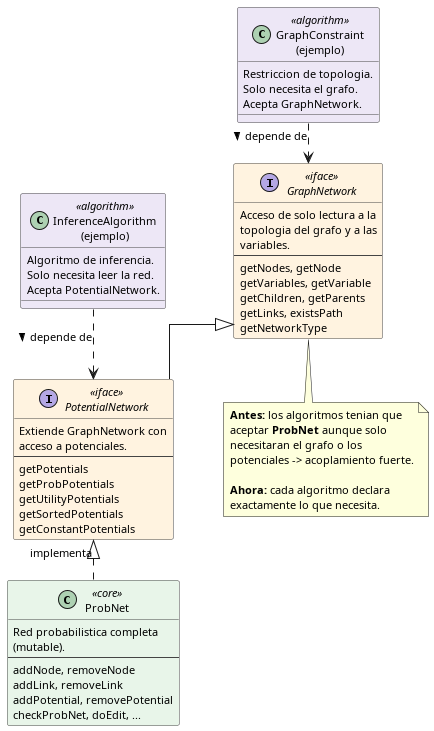
\includegraphics[width=0.7\textwidth]{interfaces.png}
  \caption{Jerarquía de interfaces.  Los algoritmos que solo necesitan
           el grafo dependen de \code{GraphNetwork}; los que necesitan
           potenciales, de \code{PotentialNetwork}.  \code{ProbNet}
           implementa ambas.}
  \label{fig:interfaces}
\end{figure}

\code{ProbNet} pasa de \code{extends Graph<Node>} a \code{implements
PotentialNetwork} y almacena el grafo como campo privado:

\begin{lstlisting}[caption={Cambio de herencia a composición en \texttt{ProbNet}.},
                   label=lst:herencia-composicion]
// ANTES:
public class ProbNet extends Graph<Node> implements ... {
    // hereda addVertex, removeVertex y toda la API de Graph
    // el grafo es ProbNet misma; no hay forma de ocultarlo
}

// DESPUES:
public class ProbNet implements PotentialNetwork, ... {
    // el grafo es un detalle de implementacion privado:
    private final Graph<Node> graph = new Graph<>();

    // ProbNet expone solo las operaciones con semantica de red:
    @Override
    public List<Node> getNodes() {
        return graph.getNodes();       // delega internamente
    }

    @Override
    public List<Node> getChildren(Node node) {
        return graph.getSuccessors(node);
    }

    @Override
    public List<Node> getParents(Node node) {
        return graph.getPredecessors(node);
    }
    // ...
}
\end{lstlisting}

\textbf{Efecto en las restricciones.}  Las 35~clases de restricción
(\code{PNConstraint}) declaraban \code{checkProbNet(ProbNet net, ...)}
y pasaron a \code{checkProbNet(GraphNetwork net, ...)}.  Esto redujo el
acoplamiento de 35~clases de una sola vez:

\begin{lstlisting}[caption={Restricciones desacopladas de \texttt{ProbNet}.},
                   label=lst:constraint]
// ANTES: cada restriccion dependia de la clase concreta
public class NoCycleConstraint extends PNConstraint {
    @Override
    public boolean checkProbNet(ProbNet net, List<Variable> vars) {
        // ...usa net.getNodes() y net.existsPath()...
    }
}

// DESPUES: solo necesita la interfaz de topologia
public class NoCycleConstraint extends PNConstraint {
    @Override
    public boolean checkProbNet(GraphNetwork net, List<Variable> vars) {
        // la interfaz garantiza exactamente lo que se usa
    }
}
\end{lstlisting}

\begin{nota}
\textbf{Las cinco restricciones que necesitaban \code{ProbNet} concreto.}
Cinco restricciones (\code{ModelNetworkConstraint},
\code{ProperUtilityPotentials}, entre otras) usaban operaciones que
\code{GraphNetwork} no expone, como comprobar potenciales.  Se decidió
mantener un cast interno a \code{ProbNet} dentro de estas restricciones
en lugar de ampliar la interfaz con operaciones que la mayoría no
necesita.  Es una solución pragmática que evita comprometer el diseño
general por casos excepcionales.
\end{nota}

% ===================================================================
\section{El resultado}
\label{sec:resultado}

\subsection{La nueva arquitectura}

La Figura~\ref{fig:after} muestra la arquitectura de \code{ProbNet} y sus
clases satélite después del rediseño.

\begin{figure}[H]
  \centering
  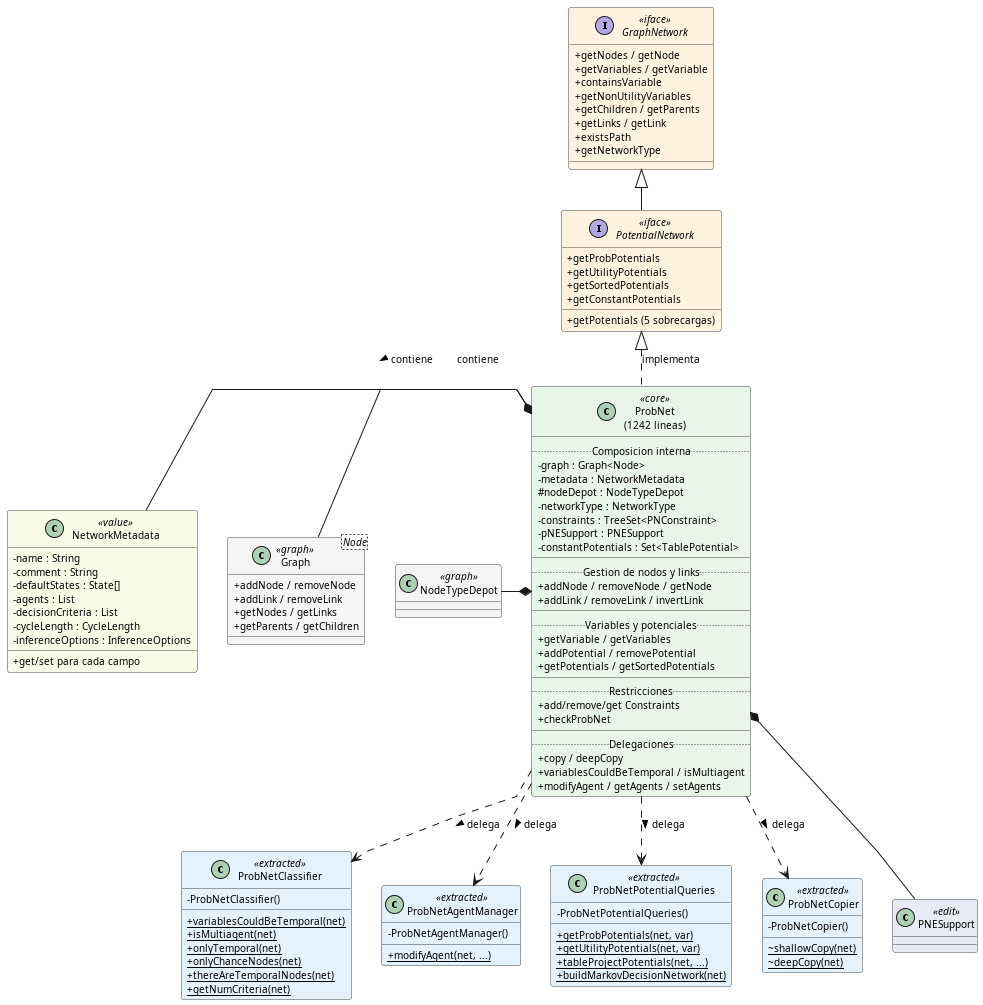
\includegraphics[width=1.1\textwidth]{after.png}
  \caption{Arquitectura de \code{ProbNet} después del rediseño (1242~líneas).
           En azul, las clases extraídas.  En naranja, las nuevas
           interfaces.  En verde y gris, los componentes de composición
           interna.}
  \label{fig:after}
\end{figure}

\subsection{Las clases extraídas}

\begin{center}
\begin{tabular}{lrp{7.5cm}}
\toprule
\textbf{Clase} & \textbf{Líneas} & \textbf{Responsabilidad} \\
\midrule
\code{GraphNetwork}              &  92 & Interfaz: vista de solo lectura del grafo. \\
\code{PotentialNetwork}          &  47 & Interfaz: extiende \code{GraphNetwork} con potenciales. \\
\code{NetworkMetadata}           &  93 & Objeto valor: todos los metadatos descriptivos. \\
\code{ProbNetCopier}             & 168 & Copia superficial y profunda de la red. \\
\code{ProbNetClassifier}         &  90 & Consultas de clasificación (6 métodos estáticos). \\
\code{ProbNetAgentManager}       &  87 & Gestión de agentes (ADD/REMOVE/RENAME/UP/DOWN). \\
\code{ProbNetPotentialQueries}   & 134 & Consultas complejas sobre potenciales. \\
\midrule
\textbf{Total nuevas clases}     & \textbf{711} & \\
\bottomrule
\end{tabular}
\end{center}

\subsection{Métricas comparadas}

\begin{center}
\begin{tabular}{lrrl}
\toprule
\textbf{Métrica} & \textbf{Antes} & \textbf{Después} & \textbf{Cambio} \\
\midrule
Líneas de \code{ProbNet.java}               & 1\,440 & 1\,242 & \good{$-$14\%} \\
Campos en \code{ProbNet}                    & 16     & 7      & \good{$-$56\%} \\
Bugs conocidos                              & 4      & 1*     & \good{$-$75\%} \\
Code smells                                 & 7      & 0      & \good{$-$100\%} \\
Restricciones acopladas a \code{ProbNet}    & 35     & 0      & \good{todas usan \code{GraphNetwork}} \\
Clases nuevas en el paquete \code{network}  & ---    & +7     & \\
Líneas totales del paquete (redistribuidas) & 1\,440 & $\sim$1\,953 & \\
\bottomrule
\end{tabular}
\end{center}

{\small * Bug B4 (\code{addShiftedNode()} sin potenciales) permanece documentado
con \code{@ToCheck} pendiente de decisión sobre el comportamiento correcto.}

La reducción de \code{ProbNet} de 1440 a 1242~líneas puede parecer pequeña
comparada con las 711~líneas de las siete clases nuevas.  El código total
del paquete creció.  Esto es el resultado esperado cuando se hace
\emph{explícito} el trabajo que una clase hacía de forma \emph{implícita}:
la God Class no era eficiente en términos de líneas; era pequeña
\emph{aparentemente} porque concentraba complejidad.  Al redistribuirla,
la complejidad se hace visible y, sobre todo, se hace \emph{dirigible}:
cada clase nueva puede mantenerse, probarse y entenderse de forma
independiente.

\subsection{Estado de ejecución de las fases}

\begin{center}
\begin{tabular}{clcl}
\toprule
\textbf{Fase} & \textbf{Descripción} & \textbf{Riesgo} & \textbf{Estado} \\
\midrule
1 & Corrección de bugs B1--B3 y smells S1--S7 & Bajo   & \good{Completada} \\
  & Extracción de \code{NetworkMetadata}       & Bajo   & \good{Completada} \\
  & Extracción de \code{ProbNetCopier}         & Bajo   & \good{Completada} \\
3 & Extracción de \code{ProbNetClassifier}     & Medio  & \good{Completada} \\
4 & Extracción de \code{ProbNetAgentManager}   & Bajo   & \good{Completada} \\
5 & Extracción de \code{ProbNetPotentialQueries} & Medio & \good{Completada} \\
  & Interfaces \code{GraphNetwork}/\code{PotentialNetwork} & Alto & \good{Completada} \\
  & Adaptar 35 restricciones a \code{GraphNetwork} & Medio & \good{Completada} \\
--& Bug B4 (\code{addShiftedNode} sin potenciales) & Bajo & \warn{Pendiente} \\
--& Mover \code{reader}/\code{writer} a la GUI    & Alto  & \warn{Pendiente} \\
\bottomrule
\end{tabular}
\end{center}

Las dos tareas pendientes son independientes del resto del rediseño.
La primera requiere consultar el comportamiento esperado en la GUI.
La segunda requiere un análisis de impacto en los módulos \code{gui} e
\code{io}.

\subsection{Qué no cambió: la API pública}

Los \textbf{490~ficheros} que referencian \code{ProbNet} no necesitaron
ninguna modificación para que los tests siguieran pasando.  Esto fue
posible gracias al patrón de delegación retrocompatible aplicado
sistemáticamente en cada extracción (§\ref{sec:hoja-ruta}).

La migración progresiva hacia las nuevas clases e interfaces es posible
pero no urgente.  Un llamador puede pasar de \code{net.isMultiagent()} a
\code{ProbNetClassifier.isMultiagent(net)} cuando lo considere conveniente,
o puede usar \code{GraphNetwork} en lugar de \code{ProbNet} en la firma de
un nuevo método.  No hay presión de tiempo.

% ===================================================================
\section{Reflexión sobre el proceso}
\label{sec:reflexion}

\subsection{Lo que facilitó la refactorización}

\paragraph{El patrón \emph{Extract Class} tenía precedente en el proyecto.}
\code{VariableTypeConverter} (extraída de \code{Node}) y
\code{VariableStateOperations} (extraída de \code{Variable}) eran
refactorizaciones del mismo tipo, hechas antes con éxito.  Tener un
precedente reduce la resistencia al cambio: la propuesta no era
especulativa, era una aplicación más del mismo patrón.

\paragraph{La retrocompatibilidad como invariante.}
Establecer desde el principio que ``la API pública no se rompe'' simplificó
la toma de decisiones.  Ante cualquier disyuntiva, la pregunta era: ¿rompe
esto alguna signatura pública existente?  Si la respuesta era sí, la
opción quedaba descartada.

\paragraph{La fase de diagnóstico por separado.}
Dedicar tiempo al análisis \emph{antes} de cambiar código produjo un
diagnóstico con bugs numerados y smells catalogados.  Cuando durante la
ejecución surgía la duda de si corregir el bug B3 dentro de la extracción
o antes, había un documento de referencia.

\subsection{Lo que fue más difícil de lo esperado}

\paragraph{El cambio de herencia a composición.}
Las 35~restricciones tuvieron que adaptarse.  La adaptación era mecánica
(cambiar el tipo del parámetro), pero ninguna herramienta de
refactorización automática del IDE pudo hacerlo de una sola vez, porque
cinco restricciones necesitaban un cast interno a \code{ProbNet} para
operaciones que \code{GraphNetwork} no expone.

\paragraph{La frontera entre \code{GraphNetwork} y \code{PotentialNetwork}.}
Decidir qué métodos pertenecen a cada interfaz requirió revisar cuáles usa
cada algoritmo de restricción.  La línea divisoria no era obvia a priori:
métodos como \code{getNonUtilityVariables()} mezclan topología (qué nodos
hay) con rol (cuáles son de utilidad).

\paragraph{Algunas correcciones son más naturales dentro de una extracción.}
El bug B3 se corrigió con más claridad dentro de \code{ProbNetAgentManager}
porque la extracción forzó un razonamiento explícito sobre el invariante de
la lista de agentes.  Corregirlo antes, dentro de la clase grande, habría
funcionado, pero habría sido más fácil introducir el mismo error de nuevo.

\subsection{Lecciones para futuros procesos de refactorización}

\begin{enumerate}
  \item \textbf{Diagnosticar antes de cambiar.}  Un diagnóstico escrito
        con bugs numerados, smells catalogados y cobertura medida acelera
        la ejecución y facilita las revisiones.

  \item \textbf{Los tests son la red de seguridad.}  Antes de extraer
        código, hay que tener tests que lo cubran.  Sin tests, la
        refactorización es potencialmente destructiva.

  \item \textbf{Pequeños pasos verificables.}  Cada fase dejó el sistema
        compilando y con todos los tests pasando.  Esto permitió detectar
        errores inmediatamente después del cambio que los causó.

  \item \textbf{La retrocompatibilidad tiene un coste que vale la pena.}
        Mantener delegaciones en \code{ProbNet} añade líneas que en un
        diseño ideal no existirían.  En un sistema con 490 dependencias,
        el coste de esas líneas es mucho menor que el de migrar 490
        ficheros de una sola vez.

  \item \textbf{La deuda técnica no resuelta debe documentarse.}  Las
        dos tareas pendientes (B4 y el smell S7) están documentadas con el
        contexto necesario para quien las aborde en el futuro.  Dejarlas
        sin resolver fue una decisión deliberada, no un olvido.
\end{enumerate}

% ===================================================================
\begin{thebibliography}{9}

\bibitem{fowler2019}
  M.~Fowler,
  \emph{Refactoring: Improving the Design of Existing Code},
  2nd~ed., Addison-Wesley, 2019.

\bibitem{martin2003}
  R.~C.~Martin,
  \emph{Agile Software Development: Principles, Patterns, and Practices},
  Prentice Hall, 2003.

\bibitem{gamma1995}
  E.~Gamma, R.~Helm, R.~Johnson, J.~Vlissides,
  \emph{Design Patterns: Elements of Reusable Object-Oriented Software},
  Addison-Wesley, 1995.

\bibitem{hunt1999}
  A.~Hunt, D.~Thomas,
  \emph{The Pragmatic Programmer},
  Addison-Wesley, 1999.

\end{thebibliography}

\end{document}
